\section{Spécifications}

\subsection{Caractérisation de l'environnement}

Il s'agit dans cette partie de caractériser l'environnement c'est-à-dire de d'identifier les entités interagissant avec le circuit à concevoir et décrire leur évolution à l'aide d'automates.
L'environnement du circuit à concevoir est constitué de trois entités :

\begin{itemize}
	\item Le processeur
	\item Le contrôleur mémoire fournissant le signal de sélection nCS\_IT.
	\item Les 15 entités informant au contrôleur d'interruptions la présence d'une interruption.
	Ce groupe d'entités est appelé "source d'interruptions".
\end{itemize}

L'ensemble processeur + contrôleur mémoire peut configurer le contrôleur d'interruptions et opérer des écritures et lectures au sein de ses registres.
Cet ensemble sera par la suite nommé "système à microprocesseur".
L'entité source d'interruptions envoie au circuit à concevoir la présence d'une interruption à traiter.

\begin{figure}[H]
	\centering
	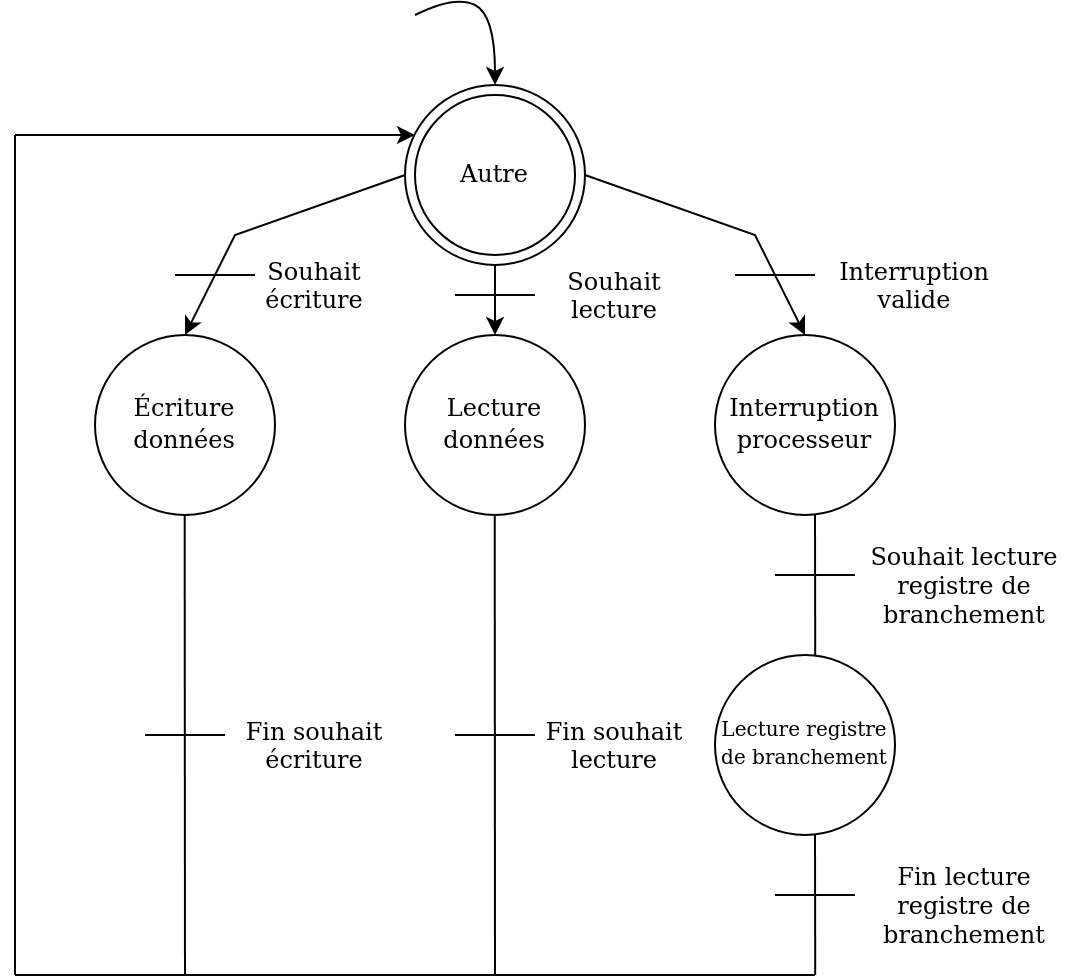
\includegraphics[width=0.8\linewidth]{figure/spec_automate_proc_ctrlmem.png}
	\caption{Comportement du système à microprocesseur}
	\label{fig:spec_automate_sysmicro}
\end{figure} 

La figure ci-dessus représente le comportement de l'entité système à microprocesseur.
Celui-ci possède trois cycles de fonctionnement.
Le processeur peut opérer des cycles de lecture et d'écriture dans les registres du contrôleur d'interruptions.
Le souhait d'écriture ou de lecture s'effectue par la mise à l'état bas du signal nCS\_IT.
La fin de ces cycles est notifiée par la mise à l'état haut du signal nAS.
Le terme "données" peut signifier la valeur des registres de configuration et également l'adresse de branchements.\\ 


\begin{figure}[H]
	\centering
	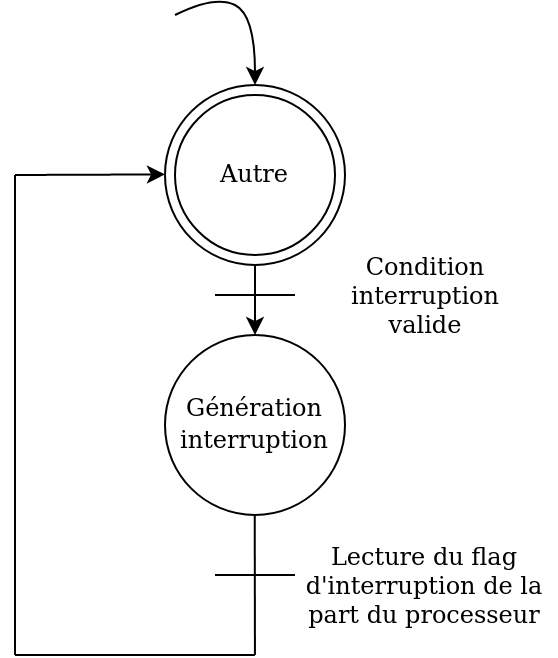
\includegraphics[width=0.5\linewidth]{figure/spec_automate_src_int.png}
	\caption{Comportement de l'entité source d'interruptions}
	\label{fig:spec_automate_src_it}
\end{figure} 

La figure ci-dessus est l'automate de l'entité source d'interruptions.
Lorsque la condition d'interruption est valide, le périphérique génère un signal en direction du contrôleur d'interruptions.
Ce signal reste actif jusqu'à la lecture du flag d'interruption de la part du processeur.

\subsection{Entrées et sorties du composant}

La caractérisation de l'environnement sous forme d'automates donne les relations d'entrées et sorties du circuit à concevoir avec les diverses entités.
Il est alors possible de présenter de manière structurelle le circuit à concevoir et les entités de l'environnement.

\begin{figure}[H]
	\centering
	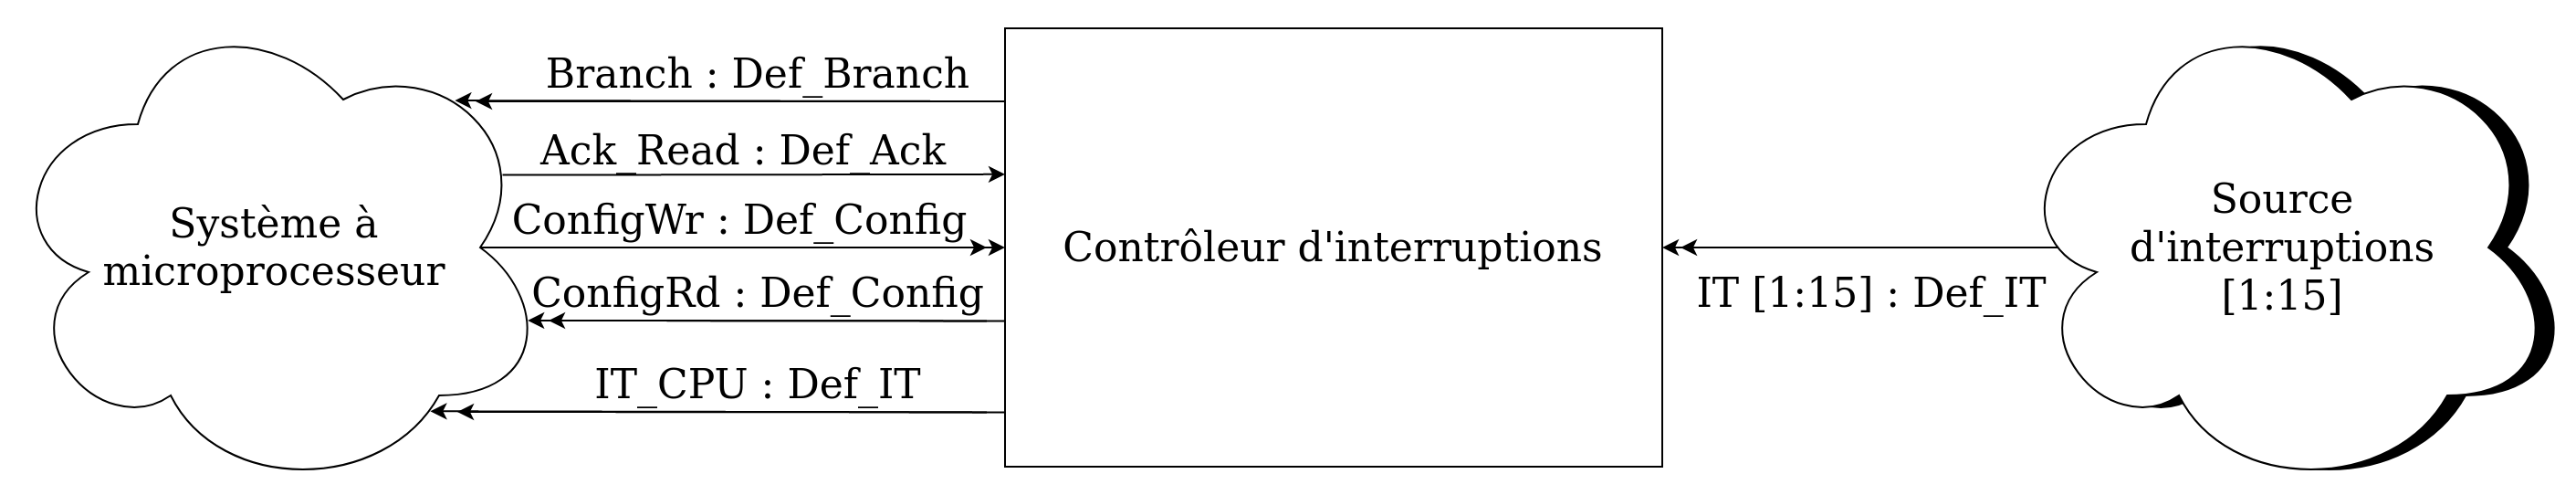
\includegraphics[width=1\linewidth]{figure/entrees_sorties_composant.png}
	\caption{Entrées et sorties du circuit à concevoir}
	\label{fig:entrees_sorties_composant}
\end{figure} 

Le tableau ci-dessous récapitule les relations avec leur sens, leur catégorie et leur type.

\begin{table}[H]
	\centering
	\begin{tabular}{|c|c|c|c|c|}
		\hline
		Entités & Relation & Catégorie & Sens & Type\\
		\hline
		& Branch & Permanent & Sortie & Def\_Branch \\
		& Ack\_Read & Évènementiel & Entrée & Def\_Ack \\
		Système à microprocesseur & ConfigWr & Permanent & Entrée & Def\_ConfigWr \\
		& ConfigRd & Permanent & Sortie & Def\_ConfigRd \\
		& IT\_CPU & Permanent & Sortie & Def\_IT\\
		\hline
		Source d'interruptions [1:15] & IT [1:15] & Permanent & Entrée & Def\_IT\\
		\hline
	\end{tabular}
	\caption{Sens et rôle des signaux}
	\label{tab:entrees_sorties_composant}
\end{table}

La relation Ack\_Read est de type Def\_Ack, une donnée de type booléen (true : la lecture de l'adresse de branchement est terminée, false sinon).
IT[1:15] est un tableau de 15 éléments de type Def\_IT, une donnée de type booléen (true : une interruption est reçu de la part de n-ième l'IP, false sinon).
IT\_CPU est également de type Def\_IT (true : une interruption doit être traitée par le CPU, false sinon).
Chaque autre relation est une composition de sous-relations comme définie ci-après.

\begin{equation*}
\mbox{Branch} = \mbox{ ID } + \mbox{ @blx }
\end{equation*}

\begin{equation*}
\mbox{ConfigWr} = \mbox{ @blx } + \mbox{ priorité } + \mbox{ masque }
\end{equation*}

\begin{equation*}
\mbox{ConfigRd} = \mbox{ ID } + \mbox{ @blx } + \mbox{ priorité } + \mbox{ masque } + \mbox{ pending } + \mbox{ traitement }
\end{equation*}

ID représente l'identifiant de l'interruption.
@blx est la sous-relation qui précise l'adresse de branchement de la sous-routine de l'interruption à traiter.
La relation priorité indique la priorité attribuée pour une interruption, masque précise si l'interruption est masquée ou non.
En ce qui concerne pending, il s'agit d'une sous-relation qui informe si une interruption est mise en attente pour être traitée ultérieurement.
Enfin, traitement prends en compte si une interruption a déjà été traitée ou non avant que celle-ci soit clear par l'IP concernée.

\begin{table}[H]
	\centering
	\begin{tabular}{|c|c|c|}
		\hline
		Sous-relation & Type & Donnée \\
		\hline
		& & \\
		ID & Def\_ID & Entier de 0 à 14\\
		& & \\
		\hline
		& & \\
		@blx & Def\_@blx & Entier de 0 à $2^{22}-1$\\
		& & \\
		\hline
		& & Entier de 0 à 7\\
		priorité & Def\_priorité & 0 : le plus prioritaire\\
		& & 7 : le moins prioritaire\\
		\hline
		& & Booléen\\
		masque & Def\_masque & true : IT masquée (prise en compte)\\
		& & false : non masquée\\
		\hline
		& & Booléen\\
		pending & Def\_pending & true : IT mise en attente\\
		& & false sinon\\
		\hline
		& & Booléen\\
		traitement & Def\_traitement & true : IT à traiter\\
		& & false : IT déjà traitée\\
		\hline
	\end{tabular}
	\caption{Sous-relations et type de données}
	\label{tab:sous-relation}
\end{table}

Il est possible d'introduire une relation interne nommée infoIT. Le k-ième élément de infoIT correspond à la k-ième interruption, c'est-à-dire la valeur de ID. Cet indice k varie de 0 à 14 (0-14 représentant les 15 interruptions).

\begin{equation*}
	\mbox{infoIT[k]} = \mbox{ ID } + \mbox{ priorité } + \mbox{ masque } + \mbox{ pending } + \mbox{ traitement }
\end{equation*}

\newpage

\subsection{Spécifications fonctionnelles}
Les spécifications fonctionnelles comprennent la liste des fonctions du système
pour l'application (fonctions externes) et la description du comportement du système et
de l'environnement pour ces fonctions \cite{Calvez_2}.

\gap

La fonction première du contrôleur d'interruption est d'informer le processeur lorsqu'une interruption valide survient.
Une interruption valide est définie comme étant non masquée et de niveau suffisant pour être prise en compte.
La gestion des niveaux de priorité est la seconde fonction à considérer. 
Elle est directement induite par la première.
Une interruption en cours ne peut être interrompue que par une interruption de niveau strictement supérieur.
Lorsque le processeur acquitte la fin du traitement, les interruptions de niveaux inférieurs ou égaux peuvent être à nouveau considérées comme valides. 
Le contrôleur fournir un niveau de priorité par défaut pour chaque source.
La troisième fonction concerne le masquage des sources d'interruption individuellement.
Une source masquée ne génèrera pas de signal au processeur.
Un événement déjà en cours de traitement par le contrôleur ne pourra être masqué. %TODO à confirmer
Si un signal d'interruption est généré alors qu'il est masqué, il est ignoré, mais s'il est démasqué alors qu'il est toujours actif alors il sera pris en compte. (\hl{A confirmer})
La quatrième fonction principale spécifie le vecteur d'exception.
Le contrôleur lorsque qu'il informe le processeur doit immédiatement lui indiquer vers quelle adresse il doit brancher.
Il est possible de configurer une adresse par source.
Sa configuration doit se faire lorsque le contrôleur est désactivé.
Si aucune adresse n'est présente pour une source donnée alors une par défaut sera attribuée.

\begin{table}[H]
	\centering
	\begin{tabular}{|c|c|}
		\hline
		nom & Description \\ \hline
		fn1 & Informer le processeur \\ \hline
		fn2 & Gérer les niveaux de priorité \\ \hline
		fn3 & Masquer individuellement les sources \\ \hline
		fn4 & Configurer le vecteur d'exception \\ \hline
	\end{tabular}
	\caption{Synthèse des spécifications fonctionnelles}
	\label{tab:spe_funct}
\end{table}

Le tableau \ref{tab:spe_funct} synthétise les spécifications fonctionnelles. 
Il permet de contrôler que chaque point est bien traité tout au long de la conception. 
Il n'est cependant pas précis et devra être traité avec la description détaillée ci-dessus.

\begin{figure}[H]
	\centering
	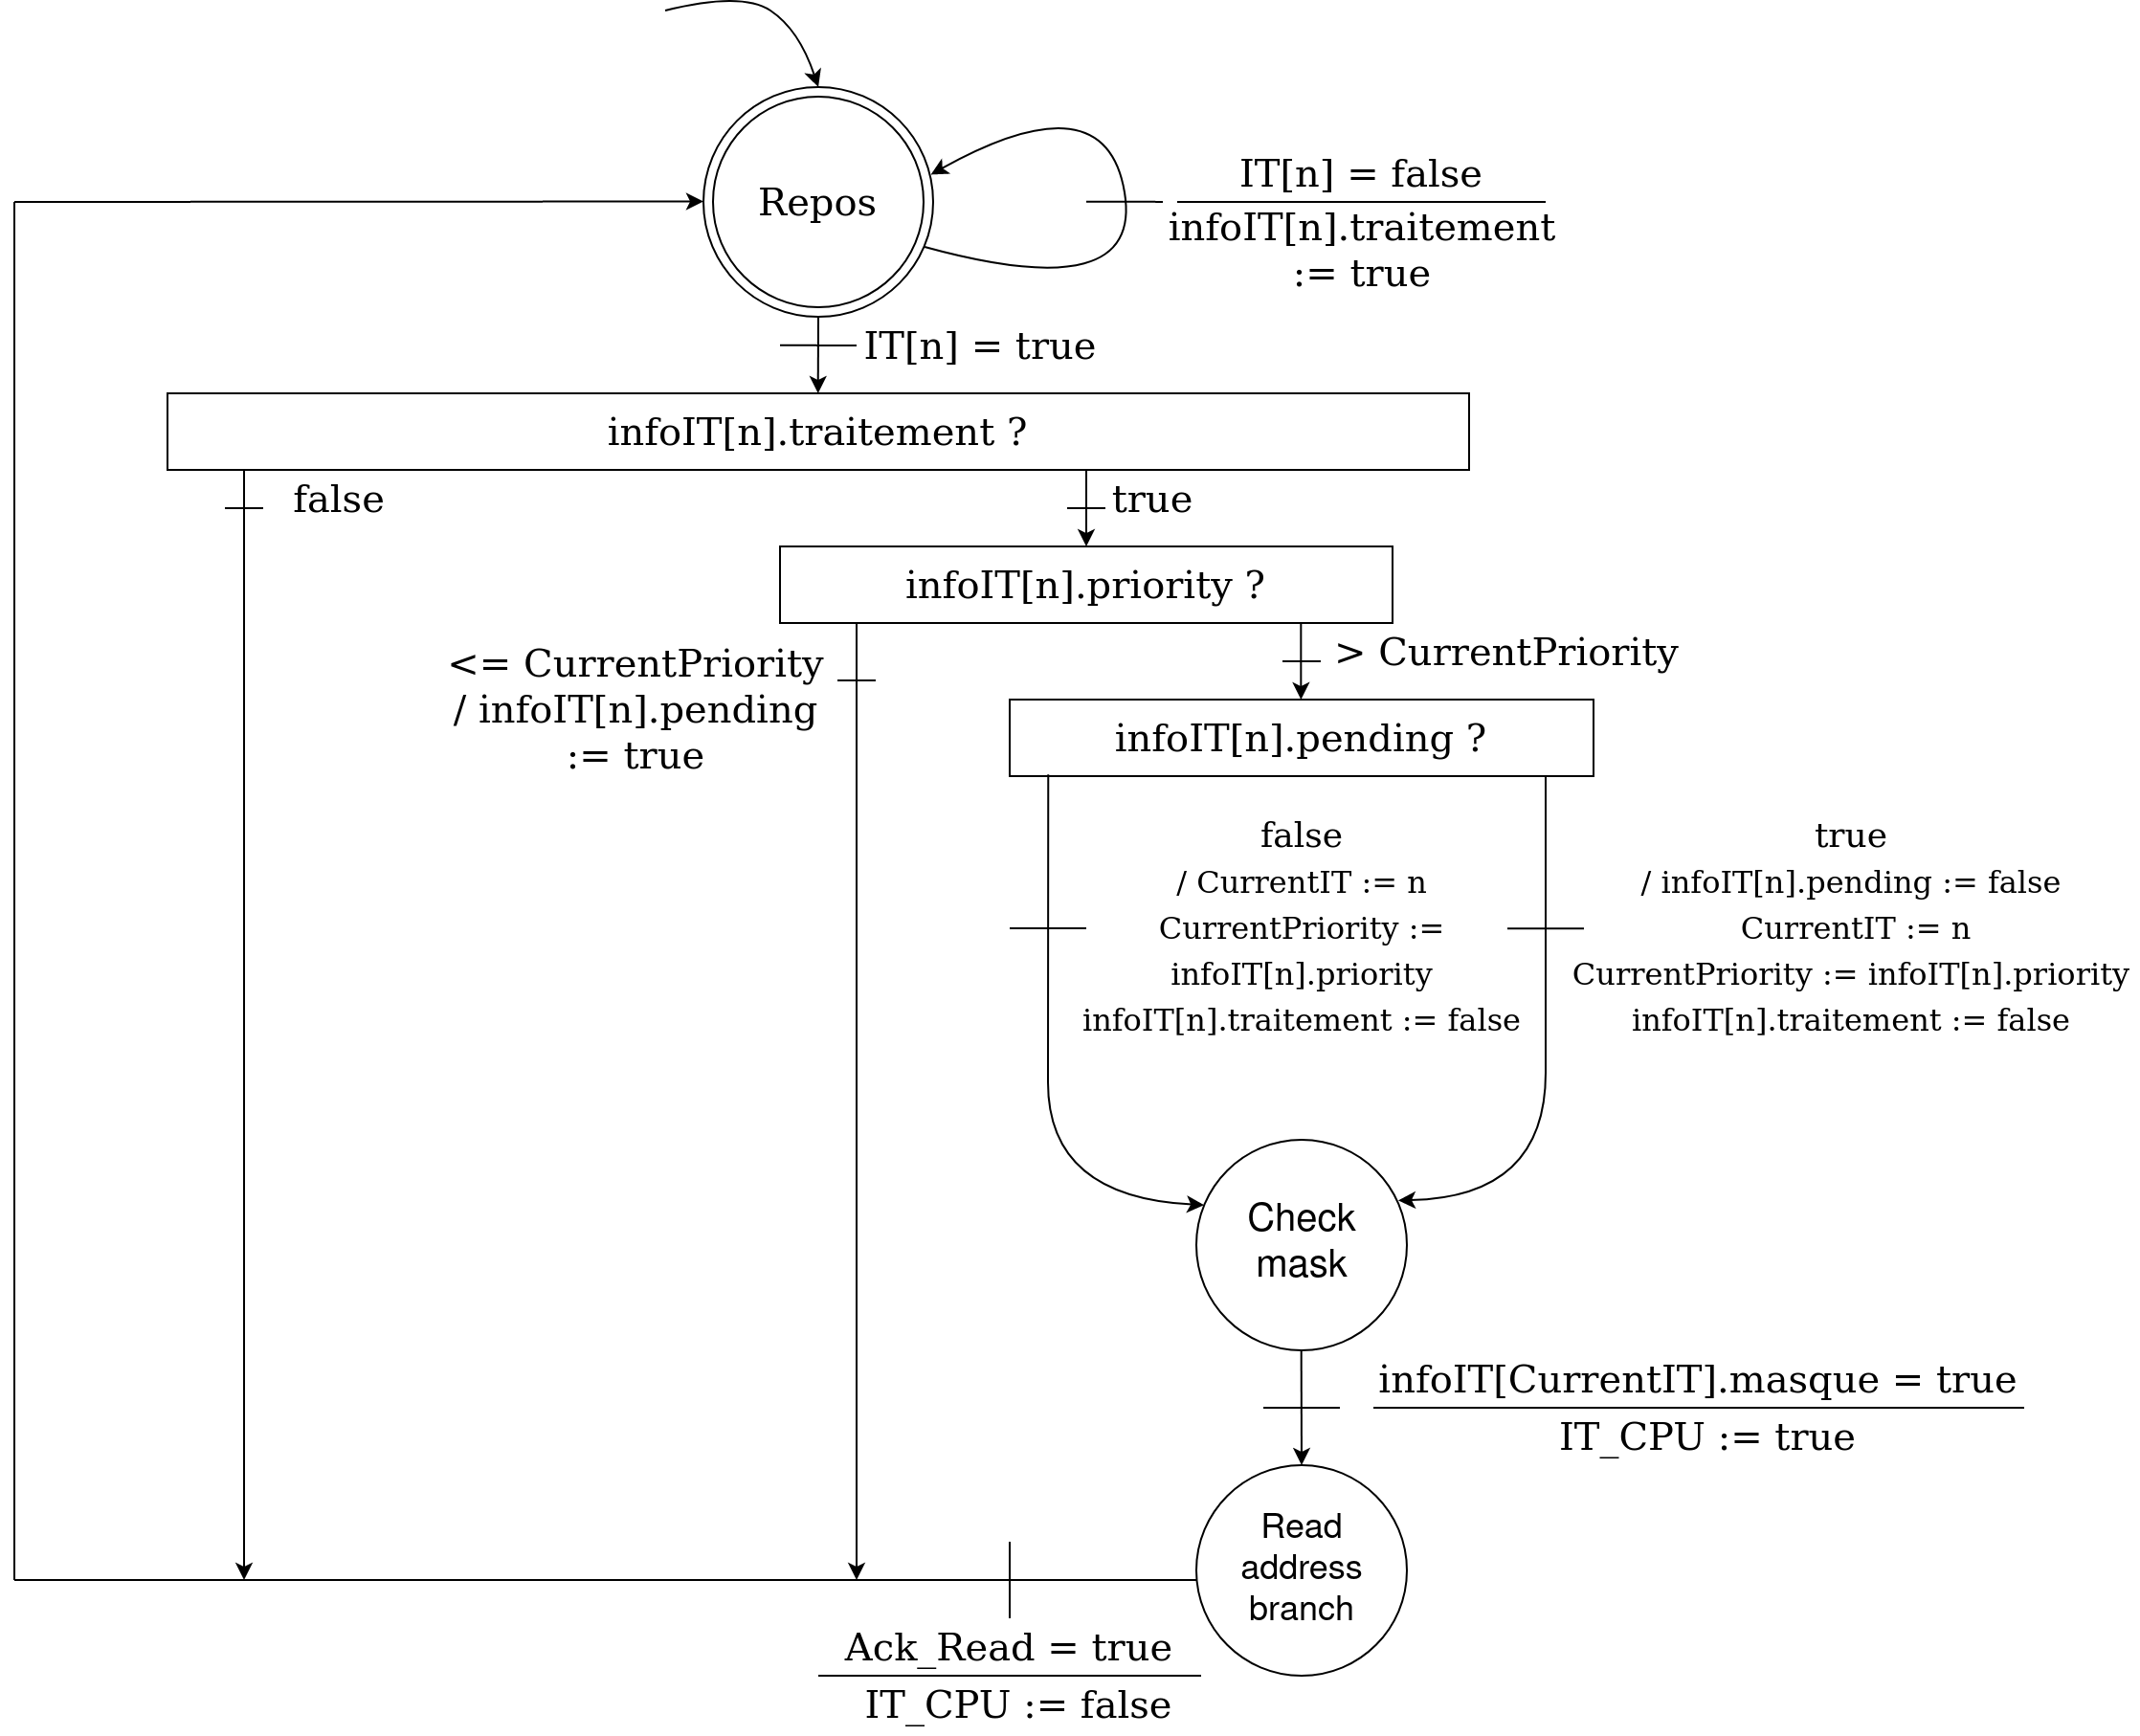
\includegraphics[width=1\linewidth]{figure/spec_fonc_1.png}
	\caption{Automate du contrôleur d'interruptions}
	\label{fig:spec_func_1}
\end{figure} 

\begin{table}[H]
	\centering
	\begin{tabular}{|c|c|c|}
		\hline
		ID & Interruptions correspondantes & Adresses de branchement par défaut\\
		\hline
		0 & nIT\_ext0 & \\
		\hline
		1 & nIT\_ext1 & \\
		\hline
		2 & nIT\_ext2 & \\
		\hline
		3 & nIT\_ext3 &\\
		\hline
		4 & nIT\_RTC &\\
		\hline
		5 & nIT\_TC\_PWM &\\
		\hline
		6 & nIT\_pos\_vit &\\
		\hline
		7 & nIT\_FFTA &\\
		\hline
		8 & nIT\_NNA &\\
		\hline
		9 & nIT\_SPI &\\
		\hline
		10 & nIT\_PCI &\\
		\hline
		11 & nIT\_UART &\\
		\hline
		12 & nIT\_I2C &\\
		\hline
		13 & nIT\_CAN &\\
		\hline
		14 & nIT\_DMA &\\
		\hline
	\end{tabular}
	\caption{Vecteurs d'interruptions}
	\label{tab:vec_int}
\end{table}

%\begin{figure}[H]
%	\centering
%	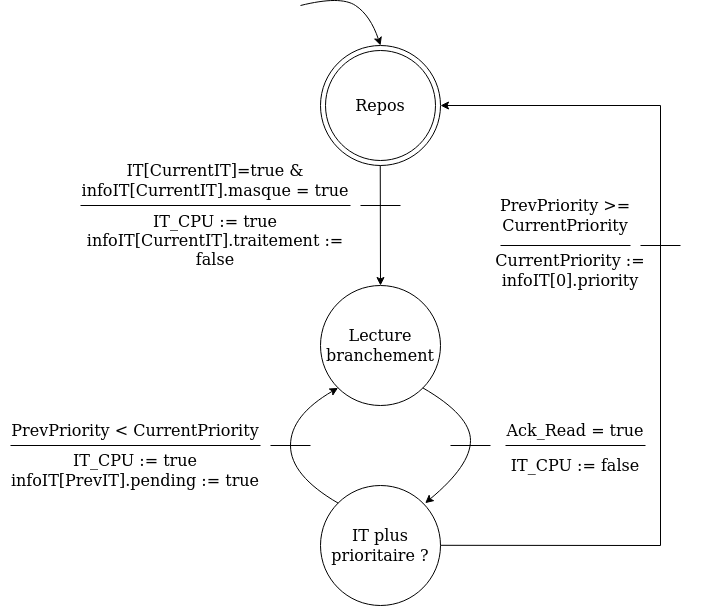
\includegraphics[width=0.9\linewidth]{figure/spec_fonc_2.png}
%	\caption{Second automate du contrôleur d'interruptions}
%	\label{fig:spec_func_2}
%\end{figure} 

\subsection{Spécification des registres}

\begin{figure}[H]
	\centering
	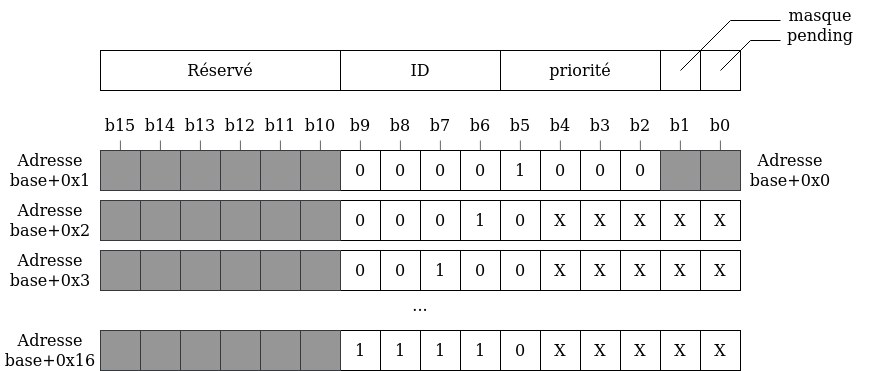
\includegraphics[width=1\linewidth]{figure/plan_registres.png}
	\caption{Organisation des registres internes}
	\label{fig:plan_registres}
\end{figure} 

\begin{figure}[H]
	\centering
	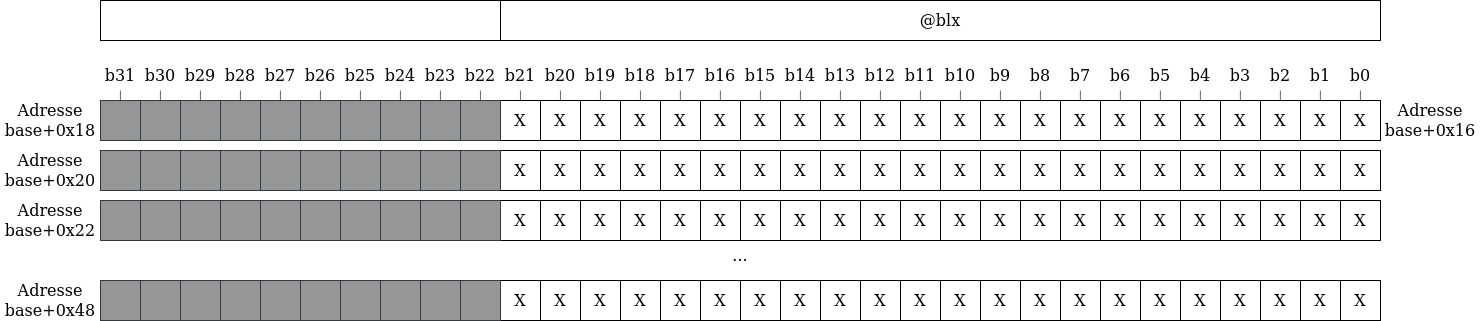
\includegraphics[width=1\linewidth]{figure/plan_branchement.png}
	\caption{Organisation du registre de branchement}
	\label{fig:plan_branchement}
\end{figure} 

\subsection{Écriture des procédures de base pour l'emploi du circuit}

(Du C à écrire (faire une lib low-level) je te laisse le plaisir de le faire)\\

\subsection{Spécifications opératoires}
\subsection{Spécifications technologiques}